\section{OBS TCEs}
\label{tces}
The Threshold Crossing Events, TCEs, are periodic events found in the Kepler time-series data by the Transit Planet Search (TPS) algorithm of the Kepler pipeline \citep[see][]{Twicken2016, Jenkins2017, Fanelli2011}.  The Data Release 25 TCEs were created by running the SOC 9.3 version of TPS on the data release 25, Q1--Q17 \Kepler\ PDC time-series.  For a thorough analysis of the DR25 TCEs and on TPS see \citet{Twicken2016}.  The DR25 TCEs, their ephemerides, and many metrics measured by the pipeline are available at the NASA Exoplanet Archive \citet{Aekeson2013}.  We disposition these signals into planet candidates and false positives.   Because the TCEs act as the input to our catalog, we first describe some of their properties as a whole and reflect on how they are different than the previous TCE table.

There are ??36,xxx DR25 OBS TCEs (Observed TCEs).  We have plotted their distribution in terms of both Period and MES (Multiple Event Statistic, a statistic that is similar to signal-to-noise, see \citep{}), in Figure~\label{f:tces}.  Notice an excessive number of short and long period TCEs, as well as many low MES TCEs.  For comparison, if you will excuse a bit of foreshadowing, the marginalized distribution of our planet candidate catalog is shown in red on the same figure.

\begin{figure*}
 \begin{center}
  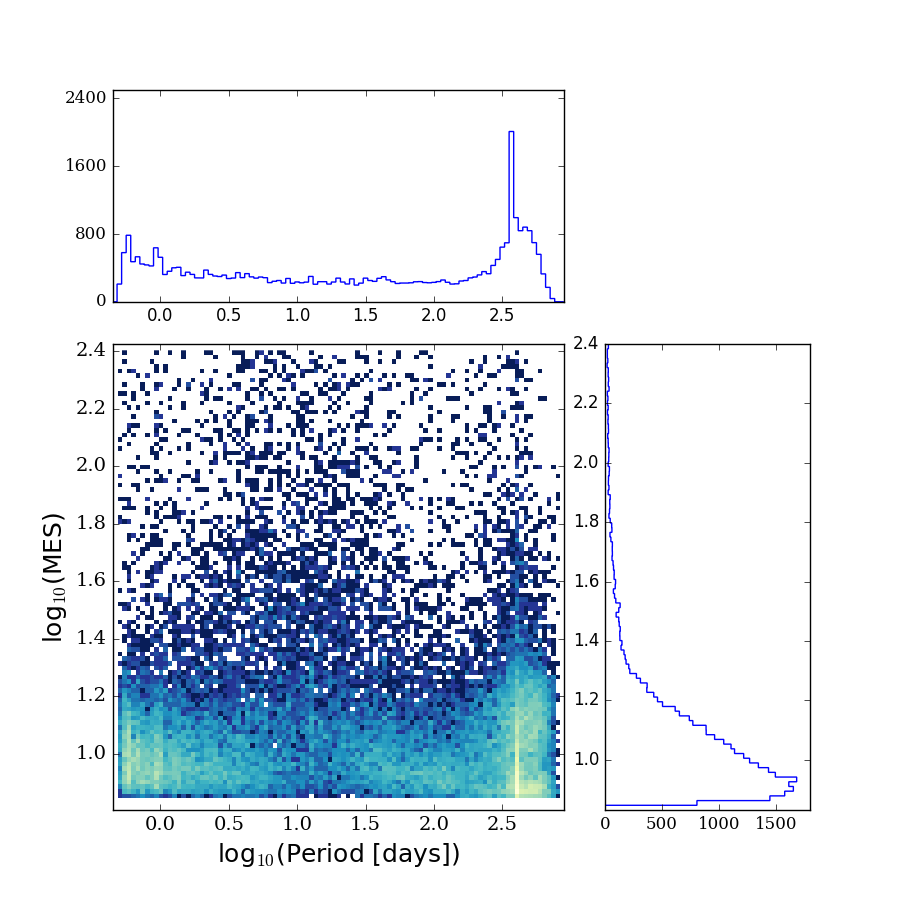
\includegraphics[width=\linewidth]{tce-dist.png}
  \caption{\ref{f:tces} A two dimensional histogram of the number of TCEs by Period and MES. A histogram of the number of TCEs by Period are projected along the x-axis and are shown at the top. A histogram of the number of TCEs by MES are projected along the y-axis and are shown on the right. For reference we show the distribution of the DR25 catalog's planet candidates in red on both the marginalized period and MES histograms.
 \end{center}

As with previous TCE catalogs, the short period ($\lt 10$\,d) excess is dominated by true, sinusoidal variability of the star. The long period excess is dominated by instrumental noise. A decrease in flux caused by a cosmic ray hit (a.k.a. SPSD, Sudden Pixel Sensitivity Drop-out), can match-up with natural fluxuations in the data to produce a TCE. Also rolling-band is highly significant on some channels \citep[see p??][]{KDCH} and since the spacecraft rolls every 90\,days, these variations can easily line-up to produce the peak at 370\,d


\end{figure*}
